\section{II : 5}
\begin{framed}\em a) What is the risk of melt-down in the power plant during a day if no observations have been made? \em\end{framed}

$$P(Meltdown) = 0.02578$$

\begin{framed}\em What if there is icy weather?\em\end{framed}

$$P(Meltdown|IcyWeather) = 0.03472$$

\begin{framed}\em b) Suppose that both warning sensors indicate failure. What is the risk of a meltdown in that case? Compare this result with the risk of a melt-down when there is an actual pump failure and water leak. What is the difference? The answers must be expressed as conditional probabilities of the observed variables, $P(Meltdown|...)$.\em\end{framed}

$$P(Meltdown|PumpFailureWarning=T,WaterLeakWarning=T) = 0.14535$$

$$P(Meltdown|PumpFailure=T,WaterLeak=T) = 0.2$$

\begin{framed}\em c) The conditional probabilities for the stochastic variables are often estimated by repeated experiments or observations. Why is it sometimes very difficult to get accurate numbers for these? What conditional probabilites in the model of the plant do you think are difficult or impossible to estimate?\em\end{framed}

Estimations are dependent on large datasets. The warnings could possibly be triggered by failure emulation, and could be fairly easy to get reliable estimates for. The weather and water leaks could be harder depending on where the power station is located, and pump failures (given that they are uncommon) would be hard to get reliable estimates for, as well as meltdowns as they are (hopefully, and usually) very rare.

\begin{framed}\em d) Assume that the "IcyWeather" variable is changed to a more accurate "Temperature" variable instead (don't change your model). What are the different alternatives for the domain of this variable? What will happen with the probability distribution of $P(WaterLeak|Temperature)$ in each alternative? \em\end{framed}

A ``generic'' $P(Temperature < 0)$ would give us a rough estimation, but more and finer ranges in common ranges would give an increased possibility for more exact estimations since a temperature of -20 most likely means that it has been cold for a longer time and will remain so for a while more, increasing the risk of waterleaks compared to a temperature of -1. This would let the probability distribution span between several discrete values rather than the current $\{.1,.2\}$. Combined with a ``over-time'' solution like the one we present on page \pageref{42}, we can increase the accuracy further, but that's another story.

\section {II : 6}
\begin{framed}\em a) What does a probability table in a Bayesian network represent?\em\end{framed}
 The probability table represent the probability of possible states in a node depending on its dependencies' states if such exists. If no dependecies, it shows the probability of possible states depending on randomness or unknown factors (such as IcyWeather: we don't know/care what actually causes---well, sub-zero temperatures, but ...--- it, we just care that it is a 5\% chance of IcyWeather).

\begin{framed}\em b) What is a joint probability distribution? Using the chain rule on the structure of the Bayesian network to rewrite the joint distribution as a product of P(child|parent) expressions, calculate manually the particular entry in the joint distribution of P(Meltdown=F, PumpFailureWarning=F, PumpFailure=F, WaterLeakWaring=F, WaterLeak=F, IcyWeather=F). Is this a common state for the nuclear plant to be in?\em\end{framed}

A joint probability distribution gives the probability of each state for given variables. For $n$ variables, each entry in an $n$-dimensional matrix represent one atomic state.
$$  P(X_1,X_2,\dots,X_n) = \prod_{i=1}^{n} P(X_i|X_{i-1},\dots,X_1) $$

\begin{align*}
  & P(\neg M, \neg PFW, \neg PF, \neg WLW, \neg WL, \neg IW) \\
  = & P(\neg M|\neg PFW, \neg PF, \neg WLW, \neg WL, \neg IW)\cdot\\
  & P(\neg PFW | \neg PF, \neg WLW, \neg WL, \neg IW)\cdot P(\neg PF | \neg WLW, \neg WL, \neg IW)\cdot\\
  & P(\neg WLW | \neg WL, \neg IW)\cdot P(\neg WL | \neg IW)\cdot P(\neg IW)\\
  = & P(\neg M | \neg PF, \neg WL)\cdot P(\neg PFW | \neg PF)\cdot P(\neg PF)P(\neg WLW | \neg WL)\cdot
  \\ & P(\neg WL | \neg IW)P(\neg IW)\\
  = & 0.999\cdot0.95\cdot0.9\cdot0.95\cdot0.9\cdot0.95 = 0.69378
\end{align*}

\begin{framed}\em c) What is the probability of a meltdown if you know that there is both a water leak and a pump failure? Would knowing the state of any other variable matter? Explain your reasoning!\em\end{framed}

The probability of $P(Meltdown|PumpFailure, WaterLeak)$ is 0.2 according to the probability table. $Meltdown$ is only conditionally dependent on $PumpFailure$ and $WaterLeak$, i.e. not dependent on any other variable. Hence, states of any other variable does not matter, which is as it should ... A warning light does not cause a meltdown, but the cause of the warning light might, and waterleaks could occur due to other reasons than frozen pipes.

\begin{framed}\em d) Calculate manually the probability of a meltdown when you happen to know that PumpFailureWarning=F, WaterLeak=F, WaterLeakWarning=F and IcyWeather=F but you are not really sure about a pump failure. \em\end{framed}
\newpage

Inference by Enumeration
$$P(X|e) = \alpha\cdot P(X,e) = \alpha\cdot\sum_{y}P(X,e,y)$$

$X = \{Meltdown\}\\E=\{PumpFailureWarning, WaterLeak, WaterLeakWarning, IcyWeather\}\\e=\{\neg pfw, \neg wl, \neg wlw,\neg iw\}\\Y=\{PumpFailure\}$
%alpha

\begin{align*}
  & \textbf{P}(X|e) = \alpha\cdot \textbf{P}(X,e) = \alpha\cdot\sum_{y}\textbf{P}(X,e,y)\\
  = & \alpha\cdot\sum_{PF}(\textbf{P}(M|PF=pf,\neg wl)\cdot
  P(\neg pfw | PF = pf)\cdot
  \textbf{P}(PF=pf)\cdot
  P(\neg wlw | \neg wl)\cdot
  P(\neg wl | \neg iw)\cdot
  P(\neg iw))\\
  = & \alpha\cdot \underbrace{P(\neg wlw | \neg wl)\cdot P(\neg wl | \neg iw)\cdot P(\neg iw)}_{\mathrm{const}}\cdot
  \sum_{pf}(\textbf{P}(M|PF = pf,\neg wl)\cdot
  P(\neg pfw|PF=pf)\cdot \textbf{P}(PF=pf))\\
  = & \alpha\cdot(\textbf{P}(M|pf,\neg wl)\cdot P(\neg pfw|pf)\cdot P(pf)
  + \textbf{P}(M|\neg pf, \neg wl)\cdot P(\neg pfw| \neg pf)\cdot P(\neg pf))\\
  = & \alpha\cdot((\langle 0.15,0.85\rangle \cdot 0.1\cdot 0.1)+(\langle 0.001, 0.999\rangle \cdot 0.95 \cdot 0.9))
  = \alpha\cdot\langle 0.00236,0.86265 \rangle\\
  = & \frac{\langle 0.00236,0.86265 \rangle}{0.00236+0.86265} = \langle 0.00272,0.99728  \rangle
\end{align*}

\section{III : 1}
\begin{framed}Model the car with the applet tool and integrate it with the model of the plant.\end{framed}

See figure \ref{figcar}.
\definecolor{ncp} {RGB}{191,255,191}
\definecolor{car} {RGB}{255,191,255}
\definecolor{bike}{RGB}{255,255,191}
\begin{figure}[h]
  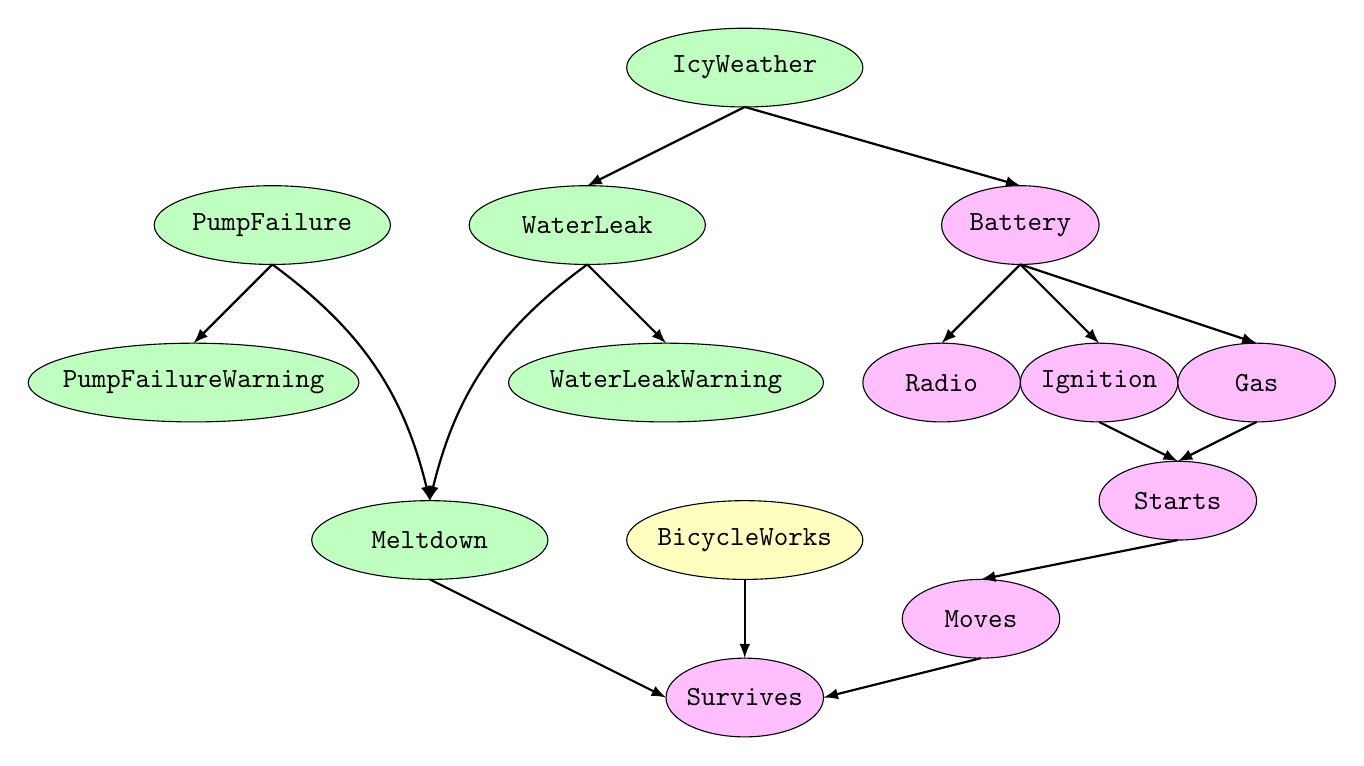
\begin{tikzpicture}

    \draw[fill=ncp] (7,9) ellipse (1.5cm and .5cm) node(a){\texttt{IcyWeather}};
    \draw[fill=ncp] (5,7) ellipse (1.5cm and .5cm) node(b){\texttt{WaterLeak}};
    \draw[fill=ncp] (1,7) ellipse (1.5cm and .5cm) node(c){\texttt{PumpFailure}};
    \draw[fill=ncp] (0,5) ellipse (2.1cm and .5cm) node(d){\texttt{PumpFailureWarning}};
    \draw[fill=ncp] (6,5) ellipse (2cm and .5cm) node(e){\texttt{WaterLeakWarning}};
    \draw[fill=ncp] (3,3) ellipse (1.5cm and .5cm) node(f){\texttt{Meltdown}};
    
    \draw[fill=car] (10.5,7) ellipse (1cm and .5cm) node(g){\texttt{Battery}};
    \draw[fill=car] (9.5,5) ellipse (1cm and .5cm) node(h){\texttt{Radio}};
    \draw[fill=car] (11.5,5) ellipse (1cm and .5cm) node(i){\texttt{Ignition}};
    \draw[fill=car] (13.5,5) ellipse (1cm and .5cm) node(j){\texttt{Gas}};
    \draw[fill=car] (12.5,3.5) ellipse (1cm and .5cm) node(k){\texttt{Starts}};
    \draw[fill=car] (10,2) ellipse (1cm and .5cm) node(l){\texttt{Moves}};
    \draw[fill=car] (7,1) ellipse (1cm and .5cm) node(m){\texttt{Survives}};

    \draw[fill=bike] (7,3) ellipse (1.5cm and .5cm) node(){\texttt{BicycleWorks}};

    \draw[arrows={-latex},thick] (7,8.5) to (5,7.5);
    \draw[arrows={-latex},thick] (5,6.5) to (6,5.5);
    \draw[arrows={-latex},thick] (5,6.5) to [bend right=20] (3,3.5);
    \draw[arrows={-latex},thick] (1,6.5) to (0,5.5);
    \draw[arrows={-latex},thick] (1,6.5) to [bend left=20] (3,3.5);
    \draw[arrows={-latex},thick] (3,2.5) to (6,1);

    \draw[arrows={-latex},thick] (7,8.5) to (10.5,7.5);
    \draw[arrows={-latex},thick] (10.5,6.5) to ( 9.5,5.5);
    \draw[arrows={-latex},thick] (10.5,6.5) to (11.5,5.5);
    \draw[arrows={-latex},thick] (10.5,6.5) to (13.5,5.5);
    \draw[arrows={-latex},thick] (11.5,4.5) to (12.5,4);
    \draw[arrows={-latex},thick] (13.5,4.5) to (12.5,4);
    \draw[arrows={-latex},thick] (12.5,3) to (10,2.5);
    \draw[arrows={-latex},thick] (10,1.5) to (8,1);

    \draw[arrows={-latex},thick] (7,2.5) to (7,1.5);

  \end{tikzpicture}
  \caption{Bayesian network for survival probability in regards of vehicle and powerplant status.}
  \label{figcar}
\end{figure}


\begin{framed}\em a) During the lunch break, the owner tries to show off for his employees by demonstrating the many features of his car stereo. To everyone's disappointment, it doesn't work. How did the owner's chances of surviving the day change after this observation?\em\end{framed}

A radio that does not work is bad mojo, it might mean that the battery is out of juice which would reduces the probability of survival. Somewhat counter-intuitive to the commons, it decreases the probability from 0.99001 to 0.98116. Bayes' Theorem gives us: $$P(Battery|\neg Radio) = \frac{P(\neg Radio|Battery)P(Battery)}{P(\neg Radio)}$$

\begin{framed}\em b) The owner buys a new bicycle that he brings to work every day. The bicycle has the following properties:
\begin{itemize}
  \item $P(BicycleWorks) = 0.9$
  \item $P(Survives | \neg Moves \land Meltdown \land BicycleWorks) = 0.6$
  \item $P(Survives | Moves \land Meltdown \land BicycleWorks) = 0.9$
\end{itemize}
How does the bicycle change the owner's chances of survival? \em\end{framed}

The bicycle adds a component of redundancy to the possibilities of escape. Adding up the numbers, the survivability from 0.99001 to 0.99505.

\begin{framed}\em c) It is possible to model any function in propositional logic with Bayesian Networks. What does this fact say about the complexity of exact inference in Bayesian Networks? What alternatives are there to exact inference? \em\end{framed}

In \emph{singly connected} Bayesian networks, the time and space complexity is linear to the size of the network. In \emph{multiply connected} networks, complexity is exponential. Alternatives to exact inference are \emph{approximate inference} methods. Using randomized samples, the accuracy is depending on the amount of generated samples.
\newpage
\section{IV : 1}
Model - see figure \ref{figHS}.
\definecolor{ncp} {RGB}{191,255,191}
\definecolor{car} {RGB}{255,191,255}
\definecolor{bike}{RGB}{255,255,191}
\begin{figure}[H]
  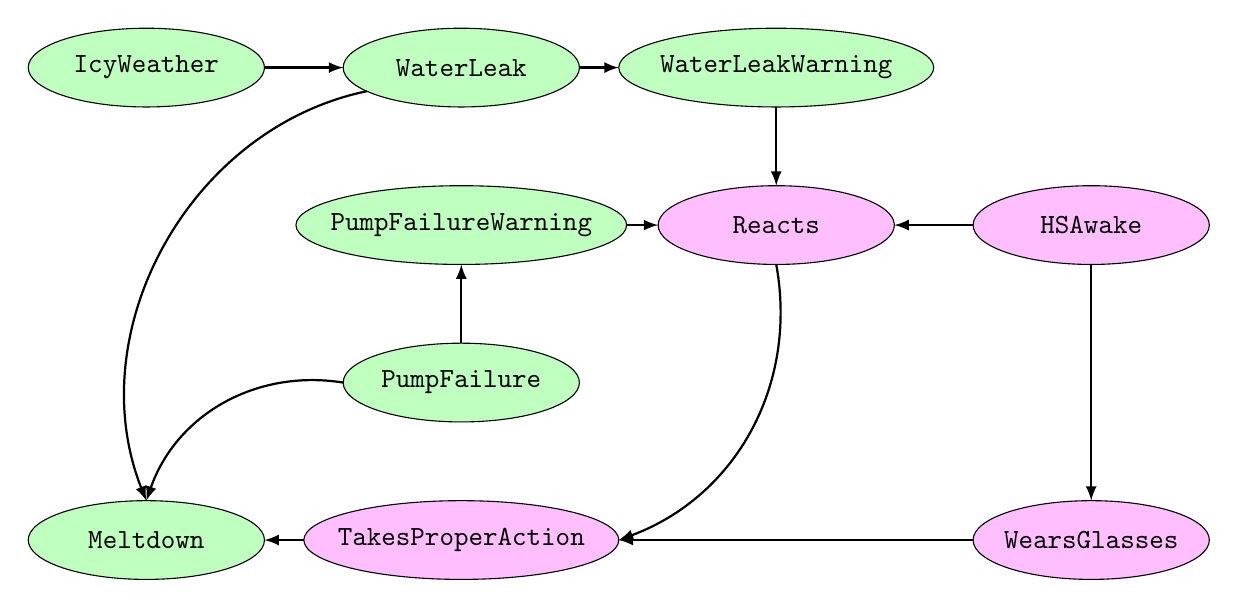
\begin{tikzpicture}

    \draw[fill=ncp] (1,4) ellipse (1.5cm and .5cm) node(a){\texttt{IcyWeather}};
    \draw[fill=ncp] (5,4) ellipse (1.5cm and .5cm) node(b){\texttt{WaterLeak}};
    \draw[fill=ncp] (5,0) ellipse (1.5cm and .5cm) node(c){\texttt{PumpFailure}};
    \draw[fill=ncp] (5,2) ellipse (2.1cm and .5cm) node(d){\texttt{PumpFailureWarning}};
    \draw[fill=ncp] (9,4) ellipse (2cm and .5cm) node(e){\texttt{WaterLeakWarning}};
    \draw[fill=ncp] (1,-2) ellipse (1.5cm and .5cm) node(f){\texttt{Meltdown}};

    \draw[fill=car] (13,2) ellipse (1.5cm and .5cm) node(){\texttt{HSAwake}};
    \draw[fill=car] (9,2) ellipse (1.5cm and .5cm) node(){\texttt{Reacts}};
    \draw[fill=car] (13,-2) ellipse (1.5cm and .5cm) node(){\texttt{WearsGlasses}};
    \draw[fill=car] (5,-2) ellipse (2cm and .5cm) node(){\texttt{TakesProperAction}};

    \draw[arrows={-latex},thick] (2.5,4) to (3.5,4);
    \draw[arrows={-latex},thick] (6.5,4) to (7,4);
%    \draw[arrows={-latex},thick] (5,3.5) to (5,2.5);
    \draw[arrows={-latex},thick] (5,0.5) to (5,1.5);
    \draw[arrows={-latex},thick] (7.1,2) to (7.5,2);
    \draw[arrows={-latex},thick] (9,3.5) to (9,2.5);
    \draw[arrows={-latex},thick] (11.5,2) to (10.5,2);
    \draw[arrows={-latex},thick] (13,1.5) to (13,-1.5);
    \draw[arrows={-latex},thick] (11.5,-2) to (7,-2);
    \draw[arrows={-latex},thick] (9,1.5) to [bend left=40](7,-2);
    \draw[arrows={-latex},thick] (3,-2) to (2.5,-2);
    \draw[arrows={-latex},thick] (3.8,3.7) to [bend right=50] (1,-1.5);
    \draw[arrows={-latex},thick] (3.5,0) to [bend right=40] (1,-1.5);


  \end{tikzpicture}
  \label{fig:car}
  \caption{Bayesian network for meltdown probability with Mr. H.S involved.}
\end{figure}


\section{IV : 2}
\begin{framed}\em The owner had an idea that instead of employing a safety person, to replace the pump with a better one. Is it possible, in your model, to compensate for the lack of Mr H.S.'s expertise with a better pump?\em \end{framed}

Yes. The probabilities of a meltdown are as follows:

\begin{tabular}{l|l|l}
  & Old Pump & New Pump\\
  w/o H.S. & 0.02578 & 0.01859\\
  with H.S & 0.02133 & N/A
\end{tabular}
\vspace{.5cm}

\begin{framed}\em Mr H.S. fell asleep on one of the plant's couches. When he wakes up he hears someone scream: "There is one or more warning signals beeping in your control room!". Mr H.S. realizes that he does not have time to fix the error before it is to late (we can assume that he wasn't in the control room at all). What is the chance of survival for Mr H.S. if he has a car with the same properties as the owner? Hint: This question involves a disjunction (A or B) which can not be answered by querying the network as is. How could you answer such questions? Maybe something could be added or modified in the network.\em\end{framed}
\vspace{.5cm}

We chose to include a node (Warning) which depends on if any warning light is observed (P=1 if so). Assuming ($\neg HSAwake$) and $Warning$ and no other observations, his survival probability would sum up to $P=0.96518$.
\vspace{.5cm}

\begin{framed}\em What unrealistic assumptions do you make when creating a Bayesian Network model of a person?\em\end{framed}
\vspace{.5cm}

  We assume the person has no sudden unforeseen medical or mental changes. Mr.HS could for example have a stroke and be unable to react to the warning lights, despite never having had a stroke before. We also assume he doesn't get better at doing his job. A few years of experience should unavoidably add to his ability to react correctly to the warning lights. In our model it does not. In the previous question we assume that he knows how to drive, and drive well enough under stress. All and all, the people in the bayesian networks covered in this lab are heavily simplified.

\vspace{.5cm}
\begin{framed}\em Describe how you would model a more dynamic world where for example the "IcyWeather" is more likely to be true the next day if it was true the day before. You only have to consider a limited sequence of days.\em\label{42}\end{framed}
\vspace{.5cm}

It would be reasonable to assume that cold enough days are not randomly distributed over the year but gathered in chunks of time which we usually refer to as ``seasons''. Hence, IcyWeather could be expanded to $n$ single connected nodes, representing the days $\{t+1, t, t-1, ... t-n\}$ where $t$ is today and let $t$ depend on previous days' observations. A $IcyWeather=T$ observation closer in time should then have a larger impact on the possibility of $IcyWeather$ for $t+1$ to be true.
